%!TEX root = ../toolhinweise.tex

\section{Nutzung des Validierungsframeworks}
\label{sec:framework}

\enlargethispage{1\baselineskip}

\begin{figure}[t]
	\centering
	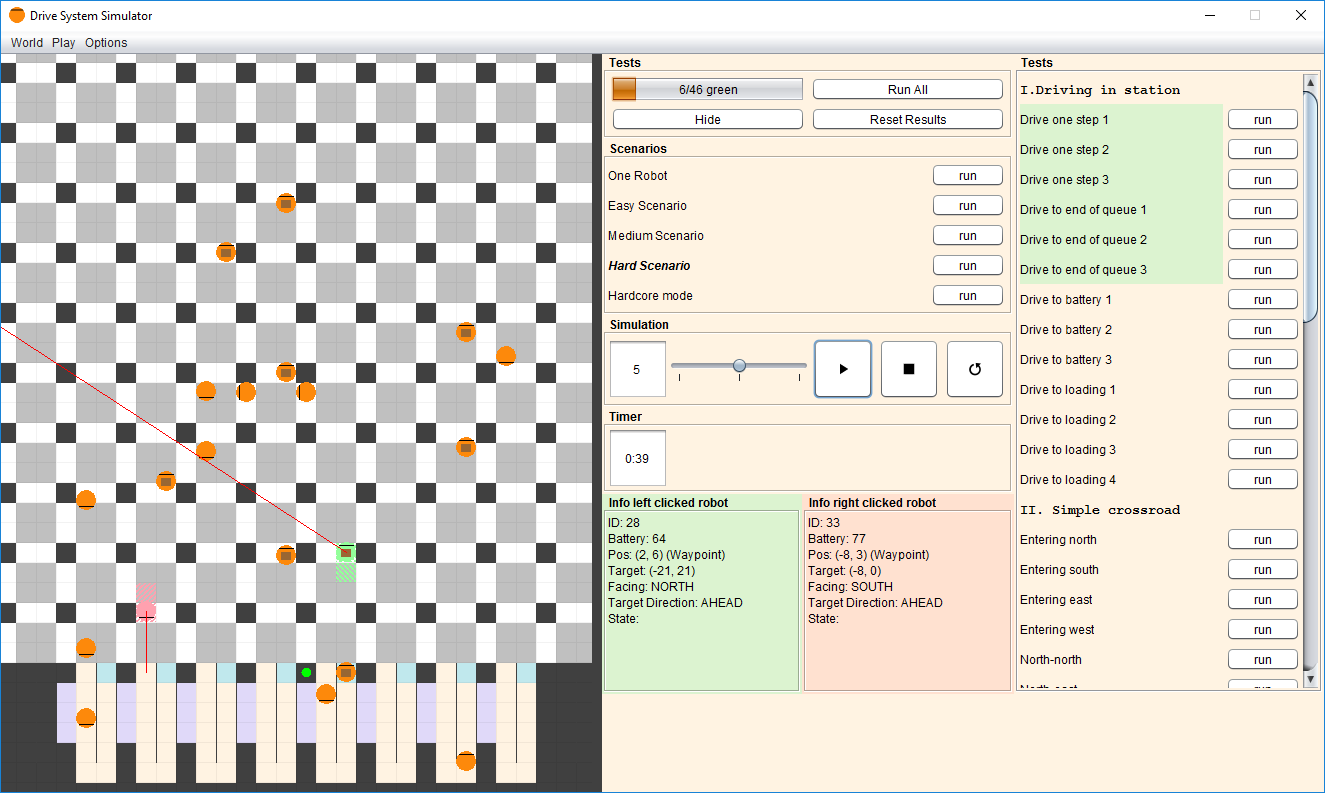
\includegraphics[width=1\textwidth]{simulator_fenster}
	\caption{Das für das \docProjectTitle{} gegebene Validierungsframework.}
	\label{fig:framework_ui}
\end{figure}


Das Validierungsframework kann gestartet werden, indem im \enquote{\red{PROJEKTNAME}}-Projekt die Datei \texttt{App.java} unter \texttt{src/de.hpi.mod.sim} ausgeführt wird. 
Dazu muss die Datei mit einem Rechtsklick angeklickt werden und im Menü \enquote{Run as} $\rightarrow$ \enquote{Java Application} ausgewählt werden. 
Für das wiederholte Ausführen ist \texttt{App.java} dann auch in der Toolbar im \enquote{Run}-Menü hinterlegt.
 
\subsection{Fenster}

Das Framework öffnet sich in einem neuen Fenster (siehe \autoref{fig:framework_ui}).
Das Fenster ist unterteilt in die \nameref{subsec:simulation} links, verschiedene Menüoptionen zum Festlegen von \nameref{subsec:settings} und Starten von \nameref{subsec:scenarios} in der Mitte sowie eine Liste an \nameref{subsec:tests} rechts.  


\subsection{Simulationsfläche}
\label{subsec:simulation}

Die Simulationsfläche bildet eine Paketsortieranlage ab, deren Struktur im Entwurfsdokument genauer beschrieben ist. 
Auf dieser Fläche bewegen sich die simulierten Roboter.

Die Größe der Simulationsfläche (und damit die Anzahl der simulierten Roboter) hängt von der Fenstergröße ab. 
Dementsprechend kann die Fenstergröße nur verändert werden, wenn gerade keine Simulation läuft.

Zur Navigation auf der Simulationsfläche können die Pfeiltasten verwendet werden.
Mit der Tastenkombination aus \enquote{Strg} und \enquote{+} bzw. \enquote{-} kann hinein- bzw. hinausgezoomt werden.


\subsection{Einstellungen}
\label{subsec:settings}

Im mittleren Teil des Fensters sind alle wichtigen Einstellungen zu finden.

Diese befinden sich insbesondere im Bereich \enquote{Simulation}. 
Dort kann per Schieberegler die Geschwindigkeit der Simulation eingestellt werden. 
Mit den benachbarten Schaltflächen kann das aktuell laufende Szenario bzw. Test pausiert, gestoppt oder neu gestartet werden. 
Zum Pausieren und Fortfahren kann auch die Leertaste verwendet werden.

Während eines laufenden Szenarios oder Tests können auf der Simulationsfläche einzelne Roboter angeklickt werden. 
Die Informationen des zuletzt mit links bzw. rechts angeklickten Roboters werden im unteren Bereich dargestellt.


\subsection{Szenarien}
\label{subsec:scenarios}

Im Bereich \enquote{Scenarios} (mitte oben) kann Simulation eines Szenarios gestartet werden. 
Je nach gewähltem Szenario, werden dabei ein oder mehrere Roboter auf der Simulationsfläche platziert.
Diese Roboter werden durch die aktuelle Version des generierten Codes gesteuert. 
Es werden kontinuierlich Aufträge an die Roboter übermittelt, bis das Szenario beendet wird. 
Kollisionen und Deadlocks führen zum vorzeitigen Abbruch des Szenarios.

Das aktuell ausgewählte Szenario ist durch eine Hervorhebung des Namens markiert.


\subsection{Tests}
\label{subsec:tests}


Ein Test prüft eine vordefinierte Fahrsituation und gibt unmittelbar eine Rückmeldung über deren Erfolg. 
Das Verhalten der Roboter kann dabei auf der Simulationsfläche beobachtet werden.

Für die Steuerung der Tests gibt es den Bereich \enquote{Tests} im mittleren Teil des Fensters sowie die Liste aller Tests im rechten Teil des Fensters. 
Die Liste aller Tests kann mit einem Klick auf \enquote{Hide} bzw. \enquote{Show} aus- bzw. eingeblendet werden.

Jeder Test kann individuell über \enquote{Run} gestartet werden. 
Alternativ kann per \enquote{Run All} die gesamte Testliste automatisch abgearbeitet werden.

Die Farbe, mit der der Titel eines Tests hinterlegt wird, gibt Auskunft über den Erfolg bzw. den Misserfolg dieses Tests beim letzten versuchten Durchlauf. 
Einen Überblick über die Testergebnisse gibt zudem der Fortschrittsbalken im Bereich \enquote{Tests}. 
Die Testergebnisse bleiben auch nach dem Schließen des Simulators erhalten, damit nicht jedes Mal die gesamte Testliste neu geprüft werden muss. 
Die Testergebnisse können mittels \enquote{Reset Results} gelöscht werden.

